\documentclass[a4paper,10pt,twocolumn]{article}

%% Language and font encodings
\usepackage[colorinlistoftodos]{todonotes}
\usepackage{arxiv}
\usepackage{subfig}
\usepackage[utf8]{inputenc} % allow utf-8 input
\usepackage[T1]{fontenc}    % use 8-bit T1 fonts
\usepackage{hyperref}       % hyperlinks
\usepackage{url}            % simple URL typesetting
\usepackage{booktabs}       % professional-quality tables
\usepackage{amsfonts}       % blackboard math symbols
\usepackage{nicefrac}       % compact symbols for 1/2, etc.
\usepackage{microtype}      % microtypography
\usepackage{lipsum}
\usepackage[title]{appendix}
\usepackage{graphicx}
\usepackage{caption}
\usepackage{graphics}
\usepackage{multirow}
\usepackage{float}
\usepackage{soul}
\usepackage{babel,blindtext}
\usepackage{booktabs}% http://ctan.org/pkg/booktabs
\newcommand{\tabitem}{~~\llap{\textbullet}~~}
%\usepackage{vmargin}
\usepackage[a4paper, inner=0.5cm, outer=0.5cm, top=0.5cm, bottom=1.5cm, bindingoffset=0.4cm]{geometry}
\usepackage{titlesec}
\titlespacing*{\section}{0.3pt}{0ex plus 1ex minus .2ex}{0ex plus .2ex}

%% Sets page size and margins
% \usepackage[a4paper,top=1cm,bottom=2cm,left=1cm,right=1cm,marginparwidth=2cm, columnsep=0.8cm]{geometry}

%% Useful packages
\usepackage{amsmath}
\usepackage{graphicx}
\usepackage[colorinlistoftodos]{todonotes}
% \usepackage[colorlinks=true, allcolors=blue]{hyperref}
% \usepackage{float}

%% Title
\title{
		%\vspace{-1in} 	
		\usefont{OT1}{bch}{b}{n}
% 		\normalfont \normalsize \textsc{ELEC6211: Project Preparation Coursework 2019/20 } \\ [10pt]
		\huge COMP6208: Advanced Machine Learning\\
}

\usepackage{authblk}
\author{
  Brent De Hauwere$^1$, Matthew De Vries$^2$, Ilias Kazantzidis$^3$, Dimitris Mallios$^4$ \\Dr. Christiaan Barnards Assistants \\
  %University of Southampton\\
  \texttt{$^1$bdh1g19, $^2$mrdv1n19, $^3$ik3n19, $^4$dm1n19}
  %\textit{*All authors contributed equally to the writing and research in this study. Their names are listed in alphabetical order.}
}
\date{}
% \affil[1]{Department of Electronics and Computer Science (ECS), University of Southampton}


\begin{document}
\maketitle

% \selectlanguage{english}



\section{Introduction}
Electrocardiogram (ECG) analysis has been established at the core of cardiovascular pathology diagnosis since its development in the twentieth century \cite{alfras}. The main problem with manual analysis of ECG signals, similar to many other time-series data, lies in difficulty of detecting and categorising different wave-forms and morphology in the signal. For a human, this task is both extensively time-consuming and prone to errors \cite{kachuee2018ecg}. 


One of the most common heart diseases which, according to the \href{https://www.nhs.uk/conditions/arrhythmia/}{NHS}, affects more than two million people every year in UK, is arrhythmia. The rhythm of the heart is controlled by electrical impulse signals. ECG monitoring can capture the cardiac signals in order to analyse abnormalities. However, the monitoring of the cardiac signals using ECG is not flawless. The signals can be interfered with additional noise (e.g muscle noise), which complicates the evaluation process and can sometimes mislead doctors into false diagnosis affecting the patient's longevity. The open access to ECG databases has led to the development of many methods and approaches for machine learning (ML) ECG arrhythmia classification over the last decade. Figure \ref{fig:heartbeat} illustrates a normal single ECG signal wave which provides useful information about the functioning of the heart.  

% \todo[inline]{This may have to go to the second part}
%Before any machine learning task it is necessary to undertake some statistical analysis in order to understand both the problem at hand as well as the dataset.
In this report we will analyse the data as well as discuss possible pre-processing and feature extraction techniques which may be used before training a model. 
\begin{figure}[ht]
     \centering
     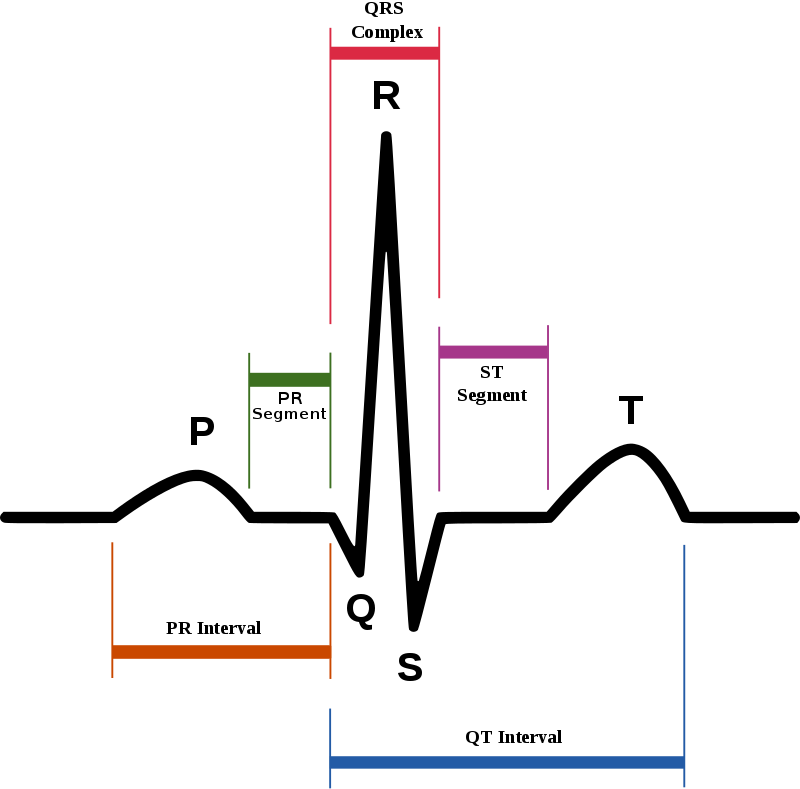
\includegraphics[height=140pt, width=0.4\textwidth]{images/heartbeat.png}
      \caption{Schematic representation of normal sinus rhythm showing normal wave, segments, and intervals [Source: \href{https://en.wikipedia.org/wiki/Sinus_rhythm}{Wikipedia}]}
      \label{fig:heartbeat}
\end{figure}

% - How is the ecg procedure done?(briefly)

% -What are arrhythmias?

% - What is the use of ml in this field? ( 1)time consuming for doctors to evaluate and 2)they also make mistakes )

% - Describe briefly fig.\ref{fig:heartbeat}

% - Describe the 5 types of arrythmias (in some papers they do it by tables)

% Most papers don't use the dataset from kaggle but the original data so we should start from there and cite \cite{moody2001impact}. One paragraph is more than enough. Not all details are needed. Things I would mention:
% - 48 half-hour excerpts(=recordings)
% - from 47 subjects(=patients)
% - from name of hospital/laboratory
% - 23 recordings randomly, 25 include clinically significant arrhythmias
% - 360 samples per second (frequency=sampling rate)
% - 2 or more cardiologists annotated each record
% - approximately 110,000 annotations at all
% Details like 11 bit - resolution, channels, leads, etc I don't believe they matter anywhere.

\section{The Dataset}
\subsection{Unprocessed Dataset}
% \hl{Electrocardiogram is an important physiological signal, which is used in assessing
% cardiac health. In general the cardiologist looks critically at the various time intervals, polarities and amplitudes of the ECG to arrive at the diagnosis.} Different features are extracted from these ECG spectra \cite{nayak}. 
The MIT-BIH dataset consists of 48 half-hour excerpts of ECG recordings from 47 different subjects recorded at the sampling rate of 360 Hz. Each beat is annotated by at least two cardiologists. This consists of 109,446 annotations of 5 categories \cite{moody2001impact}. A subsection of the labels are \cite{Clifford2007ECGA}:

\begin{itemize}
    \setlength\itemsep{0em}
    \item V — Ventricular Ectopic Beat (VEB): a ventricular premature beat, or a ventricular escape beat.
    \item F – Fusion Beat: a fusion of a ventricular and normal beat.
    \item Q — Paced Beat: a fusion of a paced and normal beat, or a beat that cannot be classified.
    \item S — Supraventricular Ectopic Beat (SVEB): an atrial or nodal (junctional) pre-mature or escape beat, or an aberrant atrial premature beat.
    \item N — Normal: any beat that does not fall into the V, F, Q, or S categories.
\end{itemize}

% First, we started by visualising the heartbeats. Figure \ref{fig:plot_beats} shows a subplot for every heartbeat category wherein each subplot contains five randomly selected beats. Notice that the amplitudes were normalised to be within the range of zero to one. From this basic visualisation, it is easy to see that beats of the same category display a similar behaviour.

% Figure \ref{fig:plot_heatmaps} shows a heatmap for each category. From these plots, we can observe strong intra-category correlations. These associations we will try to exploit with ML algorithms. 

% To look for intra-category correlations, we plotted a heatmap for every category as shown in Figure \ref{fig:plot_heatmaps}.

Figure \ref{fig:plot_heatmaps} shows a heat map for each category in order to look for intra-category correlations. In this dataset, all beats were padded to have a total of 187 samples. Therefore, we only show the first 70 samples because the colour spectrum of the graphs would be too compressed to be able to infer information otherwise. The colour of a pixel in the figure indicates how many of the beats in that respective category had a certain amplitude at a given sample number (read: point in time). In ML algorithms, these strong intra-category correlations are what we aim to exploit.

% To look for intra-category correlations, we plotted a heatmap for every category as shown in Figure \ref{fig:plot_heatmaps}. In this dataset, all beats were padded to have a total of 187 samples. Therefore, we only show the first 70 samples because otherwise the colour spectrum of the graphs would be too compressed to be able to infer information. The colour of a pixel in the figure indicates how many of the beats had a certain amplitude at a given sample number (read: point in time).

% To clarify its purpose, we analyse the subplot of the third category. From this plot, we can witness that the majority of the ventricular heartbeat signals demonstrate a normalised amplitude of 0.2 at the $20^{th}$ sample, take a downwards path, then slightly increase at the $25^{th}$ sample until the $35^{th}$ sample, whereafter they remain more or less stationary. A smaller subset of the signals start at a normalised amplitude of 0.4, show a steep increase until the $25^{th}$ sample, then decrease and eventually remain stable. In the same way, we can analyse the plots of the other categories and confirm the intra-category correlations we suspected from Figure \ref{fig:plot_beats}.

% \begin{figure}[htb]
%     \centering
%     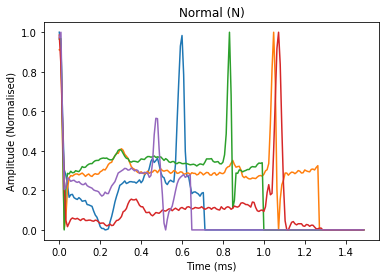
\includegraphics[width=0.19\linewidth]{images/Plot_Normal.png}
%     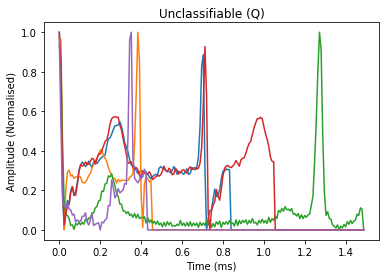
\includegraphics[width=0.19\linewidth]{images/Plot_Unclass.png}
%     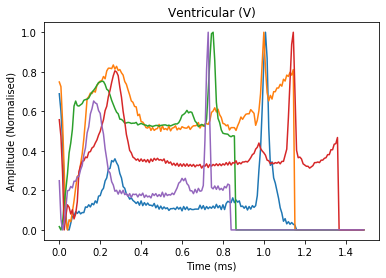
\includegraphics[width=0.19\linewidth]{images/Plot_Ventri.png}
%     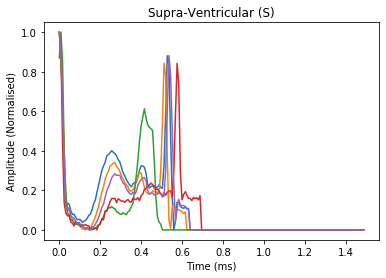
\includegraphics[width=0.19\linewidth]{images/Plot_Supra.png}
%     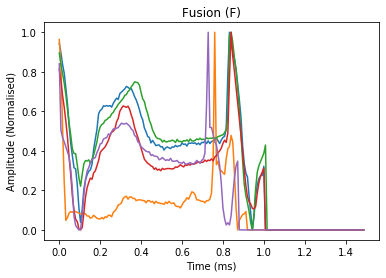
\includegraphics[width=0.19\linewidth]{images/Plot_Fusion.png}
%     \caption{5-Beat ECG for Every Category}
%     \label{fig:plot_beats}
% \end{figure}

\begin{figure}[ht]
    \centering
    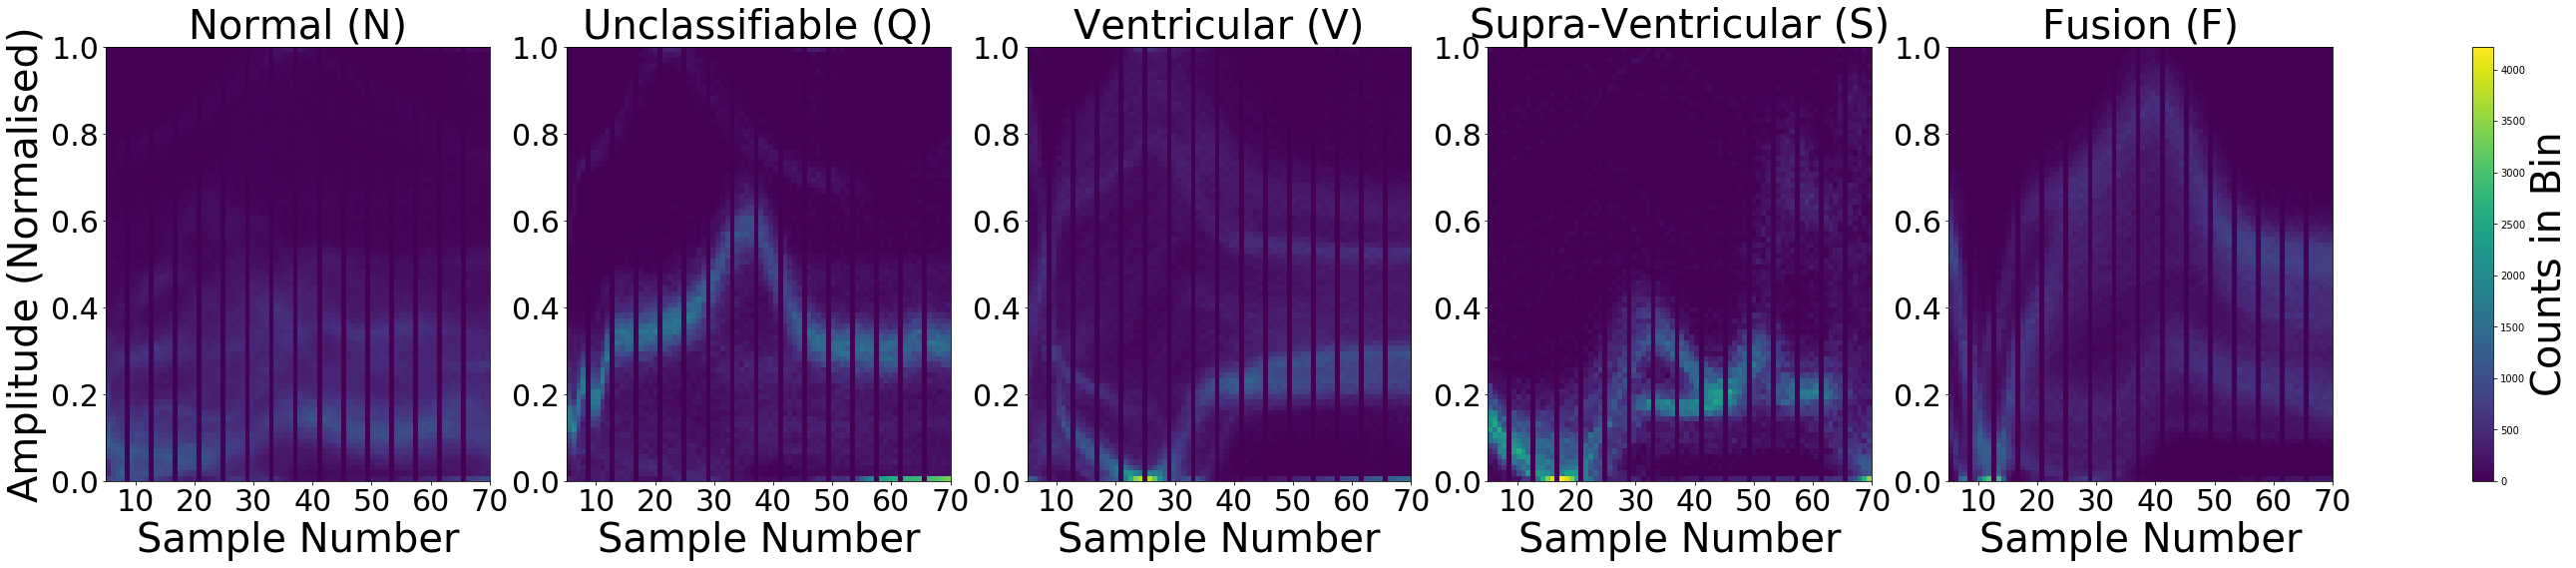
\includegraphics[width=0.95\linewidth]{images/Heatmaps.png}
    \caption{Heatmap for Every Category}
    \label{fig:plot_heatmaps}
\end{figure}

\subsection{Statistical Properties}
Several statistics can be extracted from ECG signals. We will investigate the mean and variance of the number of peaks in a signal, as well as the peak prominence. The prominence of a peak is a measure of how much a peak stands out from the surrounding baseline of the signal. It is defined as the vertical distance between the peak and its lowest contour line. Table \ref{tab:beat_features} gives an overview of the statistics for each category. We additionally calculated the average highest and top-five highest prominence value. Note that we did not take into account all prominence values because it was not informative as the majority was insignificant - diminishing the average. From this table, we can conclude that, except for category S, the mean number of peaks is not very distinguishable (which may be due to the noise). The same conclusion can be made for the average highest prominence. On the other hand, the variance in the number of peaks and the average top-five prominence's vary strongly depending on the category.

% Additionally, we will draw features from the prominence of the peaks.

% The prominence of a peak is a measure of how much a peak stands out from the surrounding baseline of the signal. It is defined as the vertical distance between the peak and its lowest contour line.


% On the other hand, the peaks in the signal are marked by orange x's. 
% \todo[inline]{Move to other section and explain prominence value. PROM OK!}

% \begin{figure}[htb]
%     \centering
%     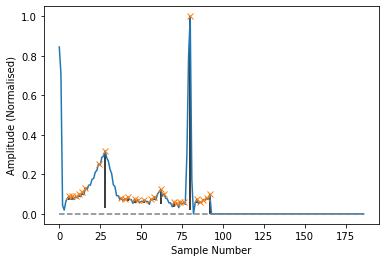
\includegraphics[width=0.7\linewidth]{images/Prominences.png}
%     \caption{Random 1-Beat ECG with Peak Prominences}
%     \label{fig:peak_prominences}
% \end{figure}



\begin{table}[h]
\centering
\begin{tabular}{|l||lllll|}
\hline
                    & N & Q & V & S  & F   \\
                     \hline
                     \hline
No. Peaks Mean      & 24.45     & 24.83     & 25.02     & 13.08     & 22.43    \\
No. Peaks Var       & 110.6    & 145.2    & 176.6    & 44     & 77.94    \\
Top-1 Prom.         & 0.64      & 0.64      & 0.64      & 0.56      & 0.70    \\
Top-5 Prom. Mean    & 0.65      & 0.24      & 0.48      & 0.52      & 0.60    \\
\hline
\end{tabular}
\caption{Intra-Category Features: Peak Mean, Peak Variance, Top-1 Prominence, and Top-5 Prominence Mean}
\label{tab:beat_features}
\end{table}


% \section*{General comments}
% This is a draft with observations and a proposed plan for the 1st report. You will understand the only parts that are written formally. I am not sure if at the 3 pages the references are included(hopefully not). I am also not quite sure if the report should be written in a very formal way as a paper with an abstract and introduction etc, or it should be written as a report with findings, what we learned etc.(we should probably ask that). Because 3 pages seem very little, we should probably use a 2 lines template and give priority to our findings and then general stuff and related work.

% This paper is the one referring to the original dataset \cite{moody2001impact}\\

% This is the thesis which has general stuff and discusses plenty of papers. It is not greatly professional, but easy to understand \cite{catalani2013arrhythmia}\\

% This is the kaggle's dataset paper. It is a good paper and we should cite it a lot because we start from the dataset which is preprocessed from those guys. \cite{kachuee2018ecg}\\

% This is probably the best, most up to date paper and understandable paper and the best to start with. \cite{alfaras2019fast}\\

% This is also very professional but it is mostly about DWT.\cite{elhaj2016arrhythmia}\\

% This is a paper you don't need to read at all because it has to do only with DWT and is not really professional \cite{emanet2009ecg}\\

% \section*{Overview (or Abstract ?)}{kachuee2018ecg
% - A brief introduction to the subject and the techniques we implemented(leave it for the end).

% \section{Principles of ECG procedure}


% The first paragraphs in the introductions of \cite{alfras} \cite{elhaj2016arrhythmia} \cite{{kachuee2018ecg} and \cite{catalani2013arrhythmia} in more detail describe these things. I think we should keep it very short and mention only things that are needed for the rest. Also don't mention yet anything about techniques of ML, other than how it can be used to the specific field.


% \todo[inline]{I think it fits more}
% \section{Overview of Methods}
\section{Related Work} 

% In the rest of this section instead of writing a part with related work which will take time to search all the related work, take space in the references, and Adam will not understand what we are talking about, we can do it better using a figure such as fig.\ref{fig:big_picture}. I sent you this figure in editable form (from draw.io) as well so you can add stuff if you want. With this figure we can talk about related work more generally, without giving very specific examples(papers) and then eliminate in the next section to what we did(fig.\ref{fig:implemented}).

Figure \ref{fig:big_picture} illustrates the most famous techniques used for the preparation of data in signal processing (specifically the ECG) ML problems. The techniques used in this research will be described in more detail in \S\ref{sec:data_exploration}. Now we will give an overview of the whole process, excluding classification which we will face in the next handin.

\begin{figure}[h]
\centering
    \centering
    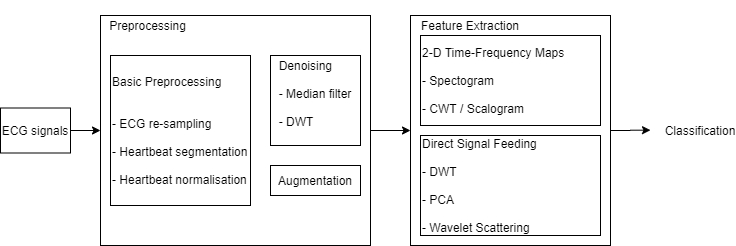
\includegraphics[width=0.4\textwidth]{images/big_picture.png}
    \captionof{figure}{Common pre-processing and feature extraction methods for ECG signals}
      \label{fig:big_picture}
\end{figure}%

Initially, some basic pre-processing has to be applied to each of the ECG signals. ECG re-sampling (specifically down-sampling) is mostly used for compression purposes and it is equivalent to the familiar process in images of resizing them to a smaller resolution. Heartbeat segmentation (and detection) is necessary for obtaining the samples. The annotations of doctors from the dataset occur at each R peak (see Figure \ref{fig:heartbeat}). Heartbeat normalisation of voltage (y axis) is also useful to keep the signal independent of the original amplitude. 

Heartbeat signals contain noise from different resources such as movement of the patients, electrodes and instrument uncertainty. Median filtering and more effectively Discrete Wavelet Transform (DWT) \cite{elhaj2016arrhythmia,emanet2009ecg} can reduce this noise and at the same time retain the useful information of the signal (P, Q, R, S, T areas). MIT-BIH arrhythmia dataset is highly imbalanced. Consequently, in order to avoid bias towards that class, techniques such as data augmentation (\S\ref{sec:data_imb}) can be used \cite{imb1, imb4}.

Regarding feature extraction, two approaches are usually followed. The first is to create 2-D time-frequency representations and tackle the signal as an image in the form of a Spectrograms (discussed in \S\ref{sec:spectograms}) which is then fed to the classifier. Scalograms are the absolute values of the Continuous Wavelet Transform (CWT) which can be additionally combined with transfer learning\footnote{A highly instructive example is presented from mathworks: \url{https://uk.mathworks.com/help/wavelet/examples/classify-time-series-using-wavelet-analysis-and-deep-learning.html}}.

The second approach is to feed signals directly to the classifier, usually after some dimensionality reduction method. In literature PCA and DWT \cite{elhaj2016arrhythmia,emanet2009ecg,catalani2013arrhythmia} are used extensively in pre-processing; the details are discussed in sections \ref{sec:4.2} and \ref{sec:4.4}. Another powerful method is the Wavelet Scattering (Invariant Scattering Convolutional Network), which is a framework of three steps in correspondence with CNNs - Convolution (Wavelets), Nonlinearity (Modulus), Averaging (Scaling Function)
- which provides low-variance features without losing critical information \cite{anden2014deep}.

\section{Data Exploration}
\label{sec:data_exploration}
Having seen the available tools from previous section, Figure \ref{fig:implemented} shows the techniques used and implemented in this research. We start with the pre-processing block.

\begin{figure}[h]
    \centering
    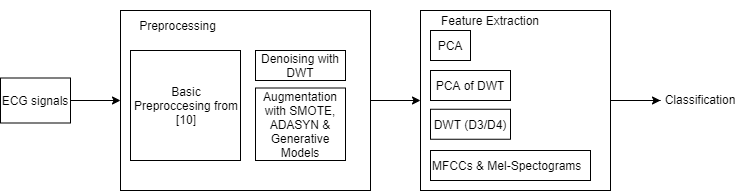
\includegraphics[width=0.5\textwidth]{images/implemented.png}
    \captionof{figure}{Our approach to pre-processing and feature extraction}
      \label{fig:implemented}
\end{figure}

\subsection{Basic Pre-processing: Adapted Dataset}
The dataset we adapted and built on\footnote{obtained on kaggle: ECG Heartbeat Categorization Dataset, \url{https://www.kaggle.com/shayanfazeli/heartbeat}}, comes from \cite{kachuee2018ecg} and the basic pre-processing applied can be easily understood from Figure \ref{fig:adapted}. The details of this approach are discussed thoroughly in \cite{kachuee2018ecg}. The main reasons why we consider it appropriate and adapt it are the following:
\begin{enumerate}
  \item The total number of samples is the same as number of annotations by doctors given in the original dataset (i.e. exactly 109,446).
%   \item It is easy to extract R-R intervals which a useful useful feature in some cases.
  \item By downsampling to 125 Hz (from 360 Hz) and zero padding, all the extracted heartbeats (observations) consist of 187 samples \footnote{samples in terms of signal processing - not ML} which is manageable for experiments with minimally affect on classification results.
%  \item As this dataset was obtained by kaggle and a lot of people have used it,  we will be able to compare the results in the exact same configuration.
  \item This basic pre-processing step does not really affect the final results. As long as all the P, Q, R, S, T parts are present in one heartbeat, and the same parts are not present in the previous or in the next sample, the information will be the same whether we segment the recording by setting the R peaks to the centre or to the edges.
\end{enumerate}

\begin{figure}[ht]
     \centering
     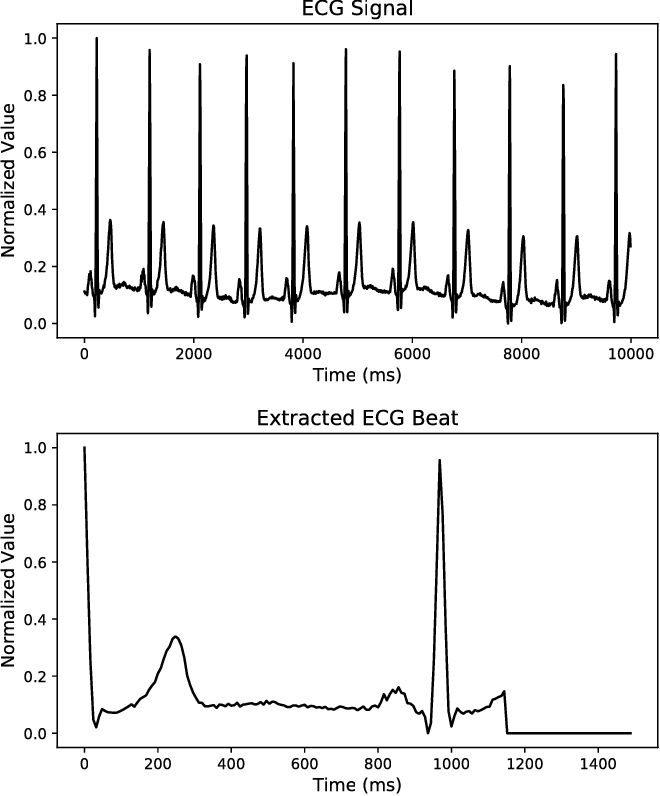
\includegraphics[width=0.3\textwidth]{images/adapted.png}
      \caption{Segmentation of heartbeat (reproduced from \cite{kachuee2018ecg})}
      \label{fig:adapted}
\end{figure}

\subsection{Data Imbalance}
\label{sec:data_imb}
% \todo[inline]{Be concise.}

ML algorithms are built to minimise errors. Since the probability of instances belonging to the majority class is significantly high in an imbalanced data set, the algorithms are much more likely to classify new observations to the majority class. With respect to classification of myocardial arrhythmia, the cost of a false negative is much larger than a false positive. There are several articles addressing the issue with imbalanced data \cite{imb1, imb3}. ML algorithms penalise false positives and false negatives equally. A way to counter this is to modify the algorithm itself to boost predictive performance on minority class. This can be executed through either recognition-based learning \cite{imb4} or cost-sensitive learning \cite{imb5}. Another approach consists of re-sampling the data in order to mitigate the effect caused by class imbalance. The re-sampling approach has gained popular acceptance among practitioners as it is more flexible and allows for the use of latest algorithms. The two most common techniques are over-sampling and under-sampling. Over-sampling increases the number of minority class members in the training set. The advantage of over-sampling is that no information from the original training set is lost, as all observations from the minority and majority classes are kept. On the other hand, it is prone to overfitting. Under-sampling, on contrary to over-sampling, aims to reduce the number of majority samples to balance the class distribution. Since it is removing observations from the original data set, it might discard useful information. Finally, one can use generative techniques in order to generate a larger data set such a General Adversarial Networks or WaveNet. Our dataset is highly imbalanced with a distribution [0.066, 0.007, 0.025, 0.073, 0.828] for [V, F, S, Q, N] respectively. We have used two over-sampling methods in this work.
% \todo[inline]{I am not sure if we need to add references about GAN or Wavenet. consider If space is available.}

% \todo[inline]{add data distribution}

\subsubsection{Synthetic Minority Over Sampling Technique (SMOTE)}
Chawla et al. \cite{smote} developed an algorithm which applies a K nearest neighbours (KNN) approach where it selects KNN, joins them and creates the synthetic samples in the space. The algorithm takes the feature vectors and its nearest neighbours and computes the distance between these vectors. The difference is multiplied by random number between (0, 1) and it is added back to feature. SMOTE algorithm is a pioneer algorithm and many other algorithms are derived from it.

% \begin{figure}
%     \centering
%     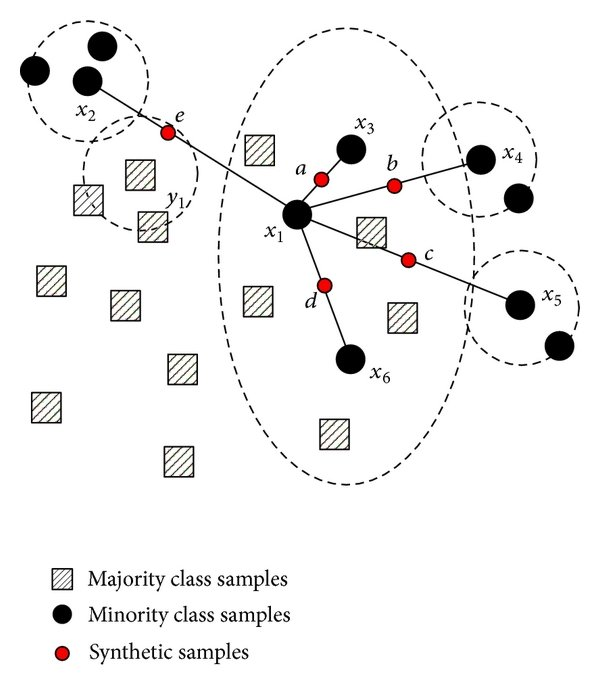
\includegraphics{images/smote.png}
%     \caption{Caption}
%     \label{fig:my_label}
% \end{figure}

\subsubsection{Adaptive Synthetic (ADASYN)}
Haibo et al. \cite{adasyn} presented a novel adaptive synthetic (ADASYN) sampling approach for learning from imbalanced data sets. The essential idea of ADASYN is to use a weighted distribution for different minority class examples according to their level of difficulty in learning, where more synthetic data is generated for minority class examples that are harder to learn compared to those minority examples that are easier to learn. As a result, the ADASYN approach improves learning with respect to the data distributions in two ways: (1) reducing the bias introduced by the class imbalance, and (2) adaptively shifting the classification decision boundary toward the difficult examples.


\subsection{Denoising with DWT}
\label{sec:4.2}
Wavelet Transform is a powerful tool used both in signals and images for denoising and feature extraction. ECG signals are non-stationary, that is, the signal changes form in time, thus the frequency spectrum changes with respect to time as well. Consequently a transform like Fourier can not capture the time changes efficiently. Short Time Fourier Transform (STFT) trades off some frequency information for time information. However, Wavelet Transform can capture both. The reason, conceptually, is that a wavelet (a zero-mean finite oscillation) is scaled and shifted through a signal and compared with the latter, in order to obtain the correlation coefficients. High scale (extension of the wavelet) captures the low frequencies of the signal and low scale (contraction of the wavelet) conversely. Consequently, the full information from both frequency and time is encoded in these correlation coefficients. The preceding procedure deflects CWT.

In DWT, the scaling and shifting is discrete (scaling uses the base of 2) and the length of coefficients is approximately the same with the input signal (less memory). The exact process is illustrated in Figure \ref{fig:dwt_filt} where high and low pass filtering is applied sequentially, and downsampling is acceptable due to Nyquist criterion. Di (detail coefficients) and Ai (approximation coefficients) represent the coefficients that encode the high and low frequency information at each level of decomposition. \footnote{description and figure about dwt were adapted by \url{https://uk.mathworks.com/help/wavelet/ref/wavedec.html} , which toolbox was used for the decomposition}

\begin{figure}[ht]
     \centering
     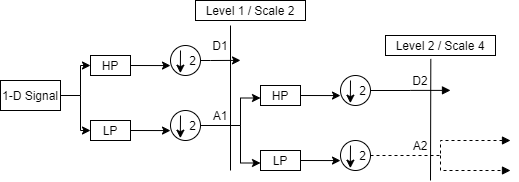
\includegraphics[width=0.4\textwidth]{images/dwt_filt.png}
      \caption{DWT decomposition} 
      \label{fig:dwt_filt}
\end{figure}

Specifically, denoising can be achieved by suitably thresholding (Universal and Soft thresholding was used) and shrinking/removing detail coefficients which include the noise towards 0. Then by reconstructing the signal from the remaining coefficients the noise will be reduced. We followed literature \cite{elhaj2016arrhythmia} which proposes 9 levels of decomposition and the Daubechies D6 wavelet. An example of the original and denoised signal is illustrated in Figure \ref{fig:den}.

\begin{figure}[ht]
     \centering
     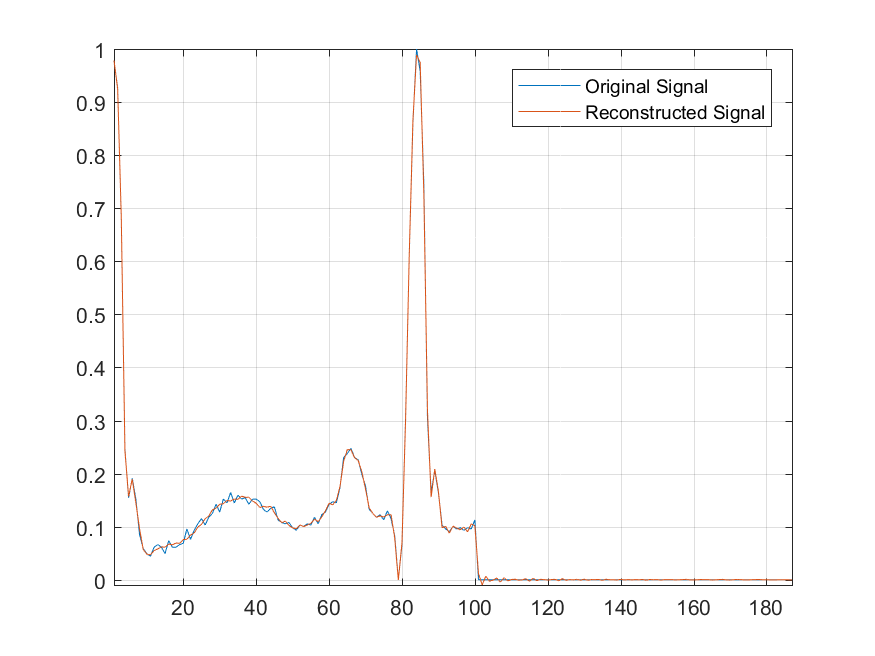
\includegraphics[width=0.35\textwidth]{images/pca.png}
      \caption{Denoising with DWT} 
      \label{fig:den}
\end{figure}

Finally, it is worth mentioning that denoising takes time and is not a compulsory step if we aim for fast automatic classifiers.



% \begin{figure}[!htb]
% \minipage{0.32\textwidth}
%   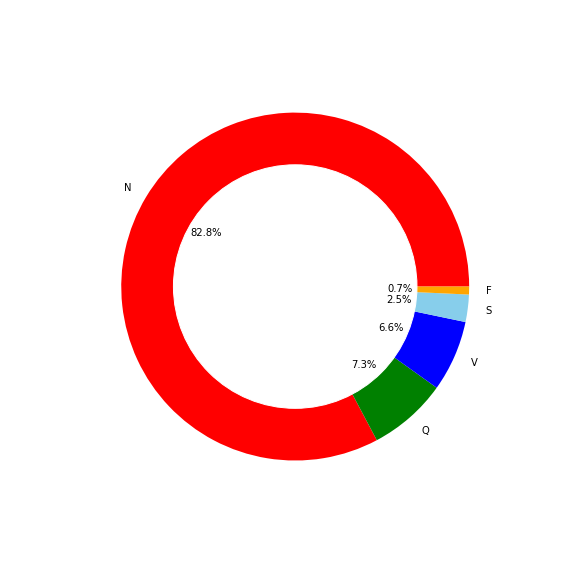
\includegraphics[width=\linewidth]{images/Unbalanced.png}
%   \caption{Original Training Set}\label{fig:awesome_image1}
% \endminipage\hfill
% \minipage{0.32\textwidth}
%   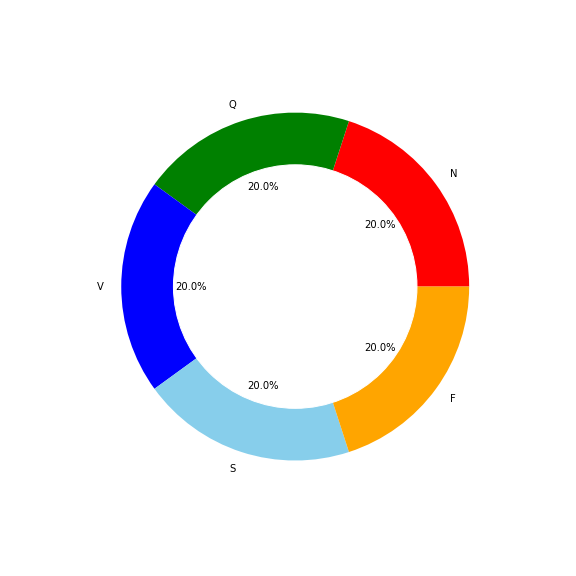
\includegraphics[width=\linewidth]{images/smotePie.png}
%   \caption{SMOTE}\label{fig:awesome_image2}
% \endminipage\hfill
% \minipage{0.32\textwidth}%
%   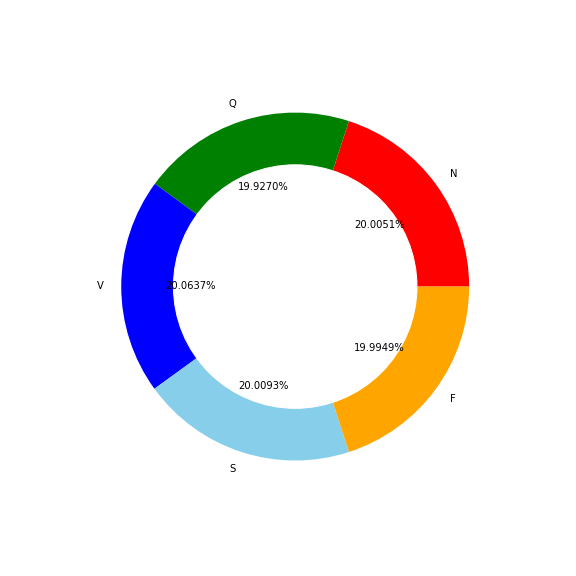
\includegraphics[width=\linewidth]{images/AdasynPie.png}
%   \caption{ADASYN}\label{fig:awesome_image3}
% \endminipage
% \end{figure}
% \nocite{*}





% \subsection{R-R intervals}
% Coming to feature extraction, it should be emphasized once again, that feature extraction is a time-consuming step and architectures aiming at online classification might omit it or add minimal features(other than the signal samples) like the R-R interval.

% Someone can continue this section. Obtaining the R-R intervals can be probably easily implemented with a threshold at 0.8-0.9, finding the 2 R peaks and getting the interval. And then adding it to the last column as a feature.

\subsection{Features from PCA and DWT}
\label{sec:4.4}
Principal Component Analysis (PCA) and DWT are predominantly used for feature extraction in ECG signals. They can be used independently or in conjunction (PCA of DWT).

Regarding only PCA, Figure \ref{fig:eigenvalues} shows how for a specific number of eigenvalues (i) used, the area under the curve and to the right of i (directions ignored) is equal to the loss of energy. We realise that we do not need all 187 features. Hence, we decided to keep 100 eigenvalues (reducing dimensions almost to the half) and observed that the reconstructed signal is almost identical to the original one.

Concerning DWT, medical research on ECG has proposed different candidate parameters and features (type of wavelet, levels of decomposition, coefficients used as features). We choose the Meyer wavelet \cite{meyer1990ondelettes}, whose shape is similar to the QRS complex (most representative part of each heartbeat\footnote{previously we had chosen db6 because the QRS complex was not a special landmark of the heartbeat in terms of denoising}) so it can capture a lot of useful information. We also choose 4 levels of decomposition as proposed in most relevant researches. In total from DWT 189 coefficients are extracted: 12 A4 + 12 D4 + 24 D3 + 47 D2 + 94 D1 (Figure \ref{fig:dwt_filt}). After that, we follow two different directions:
\begin{enumerate}
  \item Extract again 100 features with the PCA transform from all 189 DWT coefficients.
 \item Keep the detail coefficients of the third (D3) and fourth (D4) layer (i.e. 12+24=36 coefficients in total).
\end{enumerate}

\begin{figure}[ht]
     \centering
     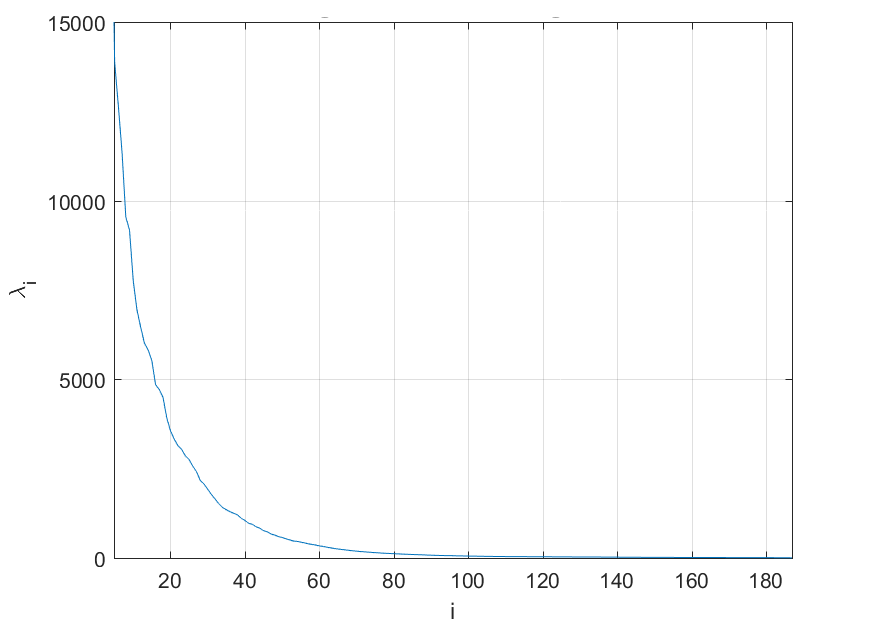
\includegraphics[width=0.33\textwidth, height=125pt]{images/eigenvalues15.png}
      \caption{Eigenvalues of a random ECG Signal} 
      \label{fig:eigenvalues}
\end{figure}


\subsection{Frequency Based Features}
\subsubsection{Mel Frequency Cepstral Coefficients}
One of the most famous feature representation methods in the field of sound and speech processing are the Mel-Frequency cepstral coefficients (MFCCs) \cite{mel_book}. The advantage of MFCCs relies on the fact that the frequency bands of the signal are distributed according to the Mel-scale. The Mel-scale is a non linear transformation method which is a good approximation of the human's auditory system instead of utilising a simple linear  model. The previous statement holds from the fact that the bands in the Mel-scale are equally spaced and as a result provide a better representation of the sound signals. ECG is basically a 1D signal similar to a sound signal but captured at a much lower frequency. %Figure \ref{fig:mfcc_block} presents the processing steps of the MFCC algorithm to produce the MFCC features. 
The dimensionality of the feature vector is 12 Mel-features per frame plus one energy feature from each frame resulting to 13 features. In this work we produce the first and the second derivatives from the MFCCs resulting to 39 features.

\subsubsection{Mel-spectrograms}
\label{sec:spectograms}
A different feature representation of the signal which is based on Mel-scale is the Mel-spectrograms. Spectrograms present the amplitude of signals at each frequency at a sequence of timesteps. Mel-Spectrograms are derived from the same algorithm as MFCC except for extracting the features after applying the Mel filter banks. The representation is a 2D binary image where the x-axis is the time and the y-axis is the frequency and each pixel has an intensity value representing the energy of the signal at each point in time at the given frequency. Audio signals are sampled in high frequency, from 16 kHz to 44 kHz using a 512-2048 size FFT window with 50\% overlap. In our problem using the rule of three and from experiment we use a FFT window size of 10 with 50\% overlap providing a 25Hz resolution regarding that our signals have low frequency. Figure \ref{fig:mel-specs} presents the Mel-spectrograms from each individual heartbeat category signals. The vivid yellow colour presents the high intensity of the signal in the corresponding frequencies while the darker purple colour presents a lower intensity respectively. The dark colours on the right of each sample occurred from the zero padding. 

% \begin{figure}[ht]
%      \centering
%      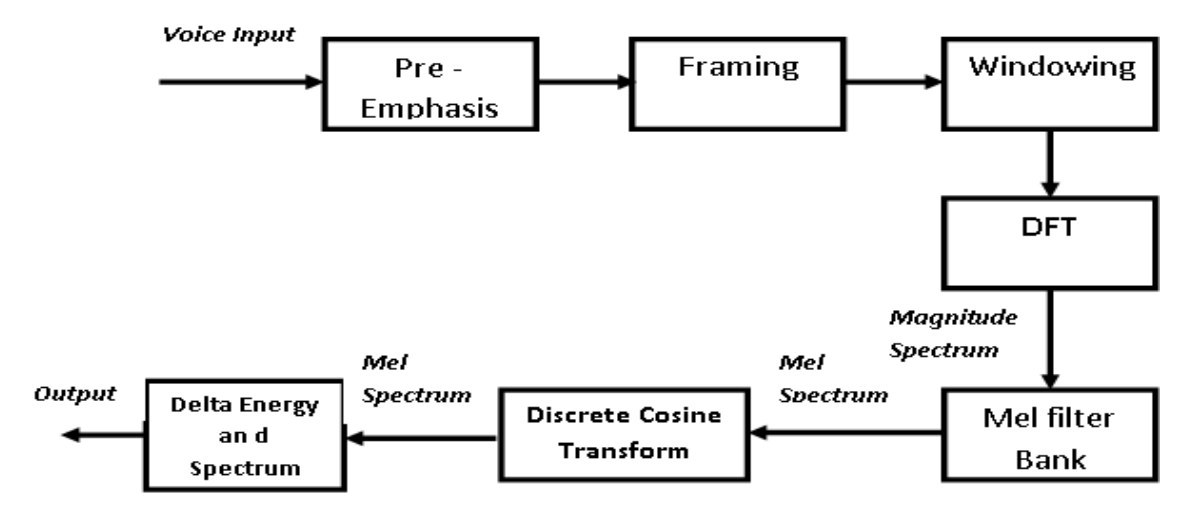
\includegraphics[width=0.42\textwidth]{images/Screenshot from 2020-03-14 02-28-57.png}
%       \caption{MFCC block diagram \cite{DBLP:journals/corr/abs-1003-4083}} 
%       \label{fig:mfcc_block}
% \end{figure}

\begin{figure}[h]
     \subfloat[N\label{fig:mel_1}]{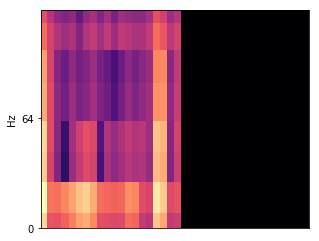
\includegraphics[width=0.09\textwidth]{images/mel_0.png}}
     \subfloat[S\label{fig:mel_2}]{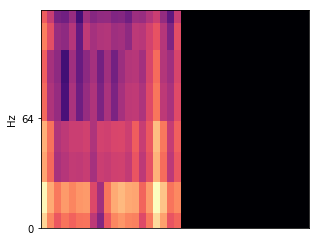
\includegraphics[width=0.09\textwidth]{images/mel_1.png}}
     \subfloat[V\label{fig:mel_3}]{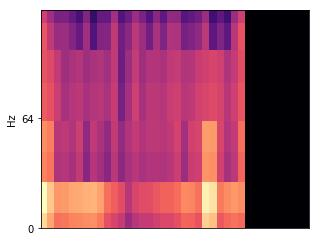
\includegraphics[width=0.09\textwidth]{images/mel_2.png}}
     \subfloat[F\label{fig:mel_4}]{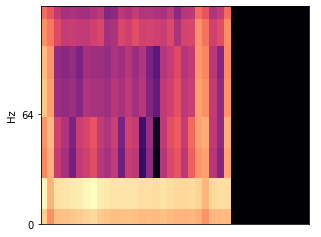
\includegraphics[width=0.09\textwidth]{images/mel_3.png}}
     \subfloat[P\label{fig:mel_5}]{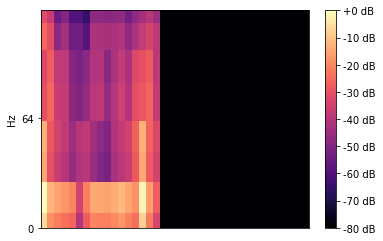
\includegraphics[height=38pt,width=0.10\textwidth]{images/mel_4.png}}
     \caption{Mel spectrogram examples from each heartbeat category.}
     \label{fig:mel-specs}
\end{figure}





\bibliographystyle{plain}
{\footnotesize
\bibliography{biblist}}


\end{document}
